\documentclass[12pt,a4paper]{report}

% =============================================================================
% BETTER Whitepaper (v2.0) — Comprehensive Technical & Economic Overview
% January 2026
%
% Compile with pdflatex (run twice for TOC/refs):
%   pdflatex BETTER_whitepaper_v2.tex
%   pdflatex BETTER_whitepaper_v2.tex
% =============================================================================

\usepackage[utf8]{inputenc}
\usepackage[T1]{fontenc}
\usepackage{lmodern}
\usepackage{microtype}
\usepackage{geometry}
\geometry{margin=1in}

\usepackage{graphicx}
\usepackage{xcolor}
\usepackage{hyperref}
\hypersetup{colorlinks=true, linkcolor=blue, urlcolor=cyan, citecolor=blue}

\usepackage{amsmath,amssymb}
\usepackage{booktabs}
\usepackage{tabularx}
\usepackage{longtable}
\usepackage{enumitem}
\setlist[itemize]{noitemsep, topsep=2pt}
\setlist[enumerate]{noitemsep, topsep=2pt}

\usepackage{tikz}
\usetikzlibrary{arrows.meta,positioning,calc,fit,shapes,backgrounds}

\usepackage{listings}
\usepackage{algorithm}
\usepackage{algpseudocode}
\usepackage{fancyhdr}
\usepackage{setspace}
\usepackage{float}
\usepackage{titlesec}
\usepackage{tocloft}

\onehalfspacing

% --- Listings configuration ---
\definecolor{codebg}{RGB}{248,248,248}
\definecolor{codegray}{RGB}{90,90,90}
\definecolor{codegreen}{RGB}{0,120,0}
\definecolor{codepurple}{RGB}{140,0,140}
\definecolor{codeblue}{RGB}{0,80,180}
\definecolor{codeorange}{RGB}{200,80,0}

% Define Rust language for listings
\lstdefinelanguage{Rust}{
  sensitive=true,
  morecomment=[l]{//},
  morecomment=[s]{/*}{*/},
  morestring=[b]",
  morestring=[b]',
  alsoletter={_:!},
  morekeywords={
    as,async,await,break,const,continue,crate,dyn,else,enum,extern,
    false,fn,for,if,impl,in,let,loop,match,mod,move,mut,pub,ref,
    return,self,Self,static,struct,super,trait,true,type,unsafe,
    use,where,while,Box,Option,Result,Some,None,Ok,Err,Vec,String,
    Arc,Mutex,RwLock,HashMap,i64,u64,f64,bool,usize
  },
  keywordstyle=\color{codeblue}\bfseries,
  commentstyle=\color{codegreen}\itshape,
  stringstyle=\color{codepurple},
}

\lstdefinelanguage{TypeScript}{
  sensitive=true,
  morecomment=[l]{//},
  morecomment=[s]{/*}{*/},
  morestring=[b]",
  morestring=[b]',
  morestring=[b]`,
  morekeywords={
    async,await,break,case,catch,class,const,continue,debugger,
    default,delete,do,else,enum,export,extends,false,finally,for,
    from,function,if,import,in,instanceof,interface,let,new,null,
    return,static,super,switch,this,throw,true,try,type,typeof,
    undefined,var,void,while,with,yield,readonly,implements,
    private,protected,public,Promise,number,string,boolean,any
  },
  keywordstyle=\color{codeblue}\bfseries,
  commentstyle=\color{codegreen}\itshape,
  stringstyle=\color{codepurple},
}

\lstset{
  backgroundcolor=\color{codebg},
  basicstyle=\ttfamily\footnotesize,
  numbers=left,
  numberstyle=\tiny\color{codegray},
  numbersep=6pt,
  frame=single,
  rulecolor=\color{black!30},
  breaklines=true,
  breakatwhitespace=false,
  showstringspaces=false,
  tabsize=2,
  captionpos=b,
  xleftmargin=1.5em,
  framexleftmargin=1em,
}

% --- Header/footer ---
\pagestyle{fancy}
\fancyhf{}
\fancyhead[L]{\footnotesize BETTER Whitepaper v2.0}
\fancyhead[R]{\footnotesize\leftmark}
\fancyfoot[C]{\thepage}
\renewcommand{\headrulewidth}{0.4pt}

% --- Convenience macros ---
\newcommand{\BETTER}{\textsc{Better}}
\newcommand{\tokenbetter}{\texttt{\$BETTER}}
\newcommand{\tokenvbetter}{\texttt{vBETTER}}
\newcommand{\code}[1]{\texttt{#1}}

% --- Title ---
\title{
  \vspace{-1cm}
  {\Huge\bfseries\BETTER}\\[0.3cm]
  {\Large Democratizing Speed in Truth-Settled Markets}\\[0.5cm]
  {\large Terminal, Vault, and Execution Rails\\for Prediction-Market Alpha}\\[1cm]
  \includegraphics[width=0.3\textwidth]{example-image-a}% Placeholder
}
\author{
  \textbf{BETTER Protocol}\\
  Whitepaper v2.0 (Draft)\\[0.5cm]
  \url{https://tradebetter.app}
}
\date{January 2026}

\begin{document}

\maketitle
\thispagestyle{empty}

\clearpage
\tableofcontents
\clearpage

% =============================================================================
\chapter*{Executive Summary}
\addcontentsline{toc}{chapter}{Executive Summary}
% =============================================================================

\section*{The Problem}

Prediction markets represent one of the most efficient mechanisms for aggregating information and producing accurate forecasts. Platforms like Polymarket have demonstrated remarkable predictive power, often outperforming traditional polling and expert analysis. However, a fundamental asymmetry exists: \textbf{informational edge decays in milliseconds}, yet retail participants lack the infrastructure to compete at machine speed.

Professional traders deploy sophisticated systems that:
\begin{itemize}
  \item Monitor multiple data feeds with sub-second latency
  \item Execute automated strategies based on real-time signals
  \item Manage risk dynamically with position sizing algorithms
  \item Aggregate alpha from diverse information sources
\end{itemize}

Retail participants, by contrast, rely on manual research, delayed information, and emotional decision-making---a structural disadvantage that compounds over time.

\section*{The BETTER Solution}

\BETTER{} is a \textbf{rails-first execution system} designed to democratize access to institutional-grade prediction market infrastructure. The protocol provides:

\begin{enumerate}
  \item \textbf{Terminal}: A high-signal operator interface for real-time market intelligence
  \item \textbf{Vault}: Pooled capital with automated strategy execution
  \item \textbf{Bounded Agents}: LLM-powered decision systems with deterministic admissibility constraints
  \item \textbf{Execution Rails}: Low-latency order routing with paper-first validation
\end{enumerate}

\section*{Key Metrics (Target)}

\begin{table}[h]
\centering
\begin{tabular}{@{}lr@{}}
\toprule
\textbf{Metric} & \textbf{Target}\\
\midrule
API latency (p50) & $<$10ms\\
Signal detection & $<$3 seconds\\
Strategy throughput & 10M+ signals/month\\
Kelly sizing precision & 0.25$\times$ fractional\\
\bottomrule
\end{tabular}
\end{table}

\clearpage

% =============================================================================
\chapter{Introduction and Thesis}
% =============================================================================

\section{The Rise of Prediction Markets}

Prediction markets have emerged as powerful tools for information aggregation. Unlike traditional financial markets, prediction market contracts settle on \textbf{objective, verifiable outcomes}---creating a direct link between price and probability.

The efficient market hypothesis suggests that prices reflect all available information. In prediction markets, this manifests as:

\begin{equation}
P(\text{outcome}) \approx \text{Market Price}
\end{equation}

When this relationship breaks down---when prices deviate from true probabilities---\textbf{alpha opportunities} emerge.

\section{The Latency Problem}

Alpha in prediction markets has an extremely short half-life. Consider a breaking news event:

\begin{enumerate}
  \item \textbf{T+0ms}: News breaks on social media
  \item \textbf{T+100ms}: Automated systems detect sentiment shift
  \item \textbf{T+500ms}: High-frequency traders adjust positions
  \item \textbf{T+2000ms}: Retail traders begin to react
  \item \textbf{T+5000ms}: Market reaches new equilibrium
\end{enumerate}

By the time a retail participant manually processes information and executes a trade, \textbf{the edge has already been arbitraged away}.

\section{Design Principles}

\BETTER{} is built on four core design principles:

\subsection{Bounded Inference}

All non-deterministic decisions (e.g., LLM-based market analysis) must produce \textbf{admissible decision records}. Malformed or unsafe outputs result in abstention rather than execution.

\begin{equation}
\text{Decision} = 
\begin{cases}
\text{Execute}(d) & \text{if } d \in \mathcal{A}_{\text{admissible}}\\
\text{Abstain} & \text{otherwise}
\end{cases}
\end{equation}

\subsection{Deterministic Execution}

The order lifecycle is engineered to be:
\begin{itemize}
  \item \textbf{Idempotent}: Duplicate submissions produce identical outcomes
  \item \textbf{Observable}: Full audit trail from signal to settlement
  \item \textbf{Risk-capped}: Hard limits on position size and exposure
\end{itemize}

\subsection{Paper-First Validation}

Every strategy runs in paper mode before live deployment, with realistic simulation of:
\begin{itemize}
  \item Latency (base + jitter)
  \item Slippage (spread crossing + market impact)
  \item Partial fills and rejections
  \item Fee structures
\end{itemize}

\subsection{Composable Architecture}

The system is designed for horizontal scaling:
\begin{itemize}
  \item Signal sources can be added without core changes
  \item Strategies are pluggable modules
  \item Execution adapters abstract venue-specific logic
\end{itemize}

\clearpage

% =============================================================================
\chapter{System Architecture}
% =============================================================================

\section{High-Level Overview}

The \BETTER{} system consists of four primary layers:

\begin{figure}[H]
\centering
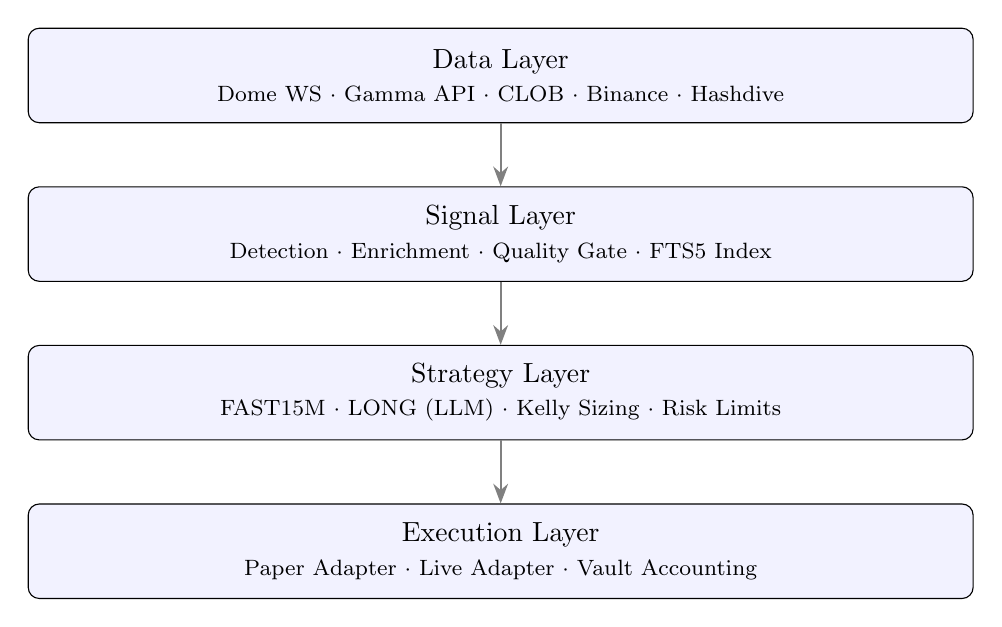
\begin{tikzpicture}[
  layer/.style={rectangle, draw, rounded corners, minimum width=12cm, minimum height=1.2cm, align=center, fill=blue!5},
  arrow/.style={-{Stealth[length=2.5mm]}, thick, gray},
  node distance=0.8cm
]

\node[layer] (data) {Data Layer\\{\footnotesize Dome WS $\cdot$ Gamma API $\cdot$ CLOB $\cdot$ Binance $\cdot$ Hashdive}};
\node[layer, below=of data] (signal) {Signal Layer\\{\footnotesize Detection $\cdot$ Enrichment $\cdot$ Quality Gate $\cdot$ FTS5 Index}};
\node[layer, below=of signal] (strategy) {Strategy Layer\\{\footnotesize FAST15M $\cdot$ LONG (LLM) $\cdot$ Kelly Sizing $\cdot$ Risk Limits}};
\node[layer, below=of strategy] (execution) {Execution Layer\\{\footnotesize Paper Adapter $\cdot$ Live Adapter $\cdot$ Vault Accounting}};

\draw[arrow] (data) -- (signal);
\draw[arrow] (signal) -- (strategy);
\draw[arrow] (strategy) -- (execution);

\end{tikzpicture}
\caption{BETTER system architecture layers}
\end{figure}

\section{Technology Stack}

\begin{table}[H]
\centering
\begin{tabular}{@{}lll@{}}
\toprule
\textbf{Component} & \textbf{Technology} & \textbf{Rationale}\\
\midrule
Backend Runtime & Rust + Tokio & Zero-cost async, memory safety\\
Web Framework & Axum & Type-safe routing, tower middleware\\
Database & SQLite (WAL) & Low-ops, 10M+ signal capacity\\
Frontend & React 18 + TypeScript & Component model, type safety\\
State Management & Zustand & Minimal boilerplate, merge-by-id\\
Real-time & WebSocket + REST & Hybrid delivery for reliability\\
\bottomrule
\end{tabular}
\caption{Technology stack}
\end{table}

\section{Application State}

The backend maintains shared state across all concurrent handlers:

\begin{lstlisting}[language=Rust, caption={Core application state structure}]
#[derive(Clone)]
struct AppState {
    signal_storage: Arc<DbSignalStorage>,
    risk_manager: Arc<ParkingRwLock<RiskManager>>,
    signal_broadcast: broadcast::Sender<WsServerEvent>,
    http_client: reqwest::Client,
    dome_rest: Option<Arc<DomeRestClient>>,
    polymarket_market_ws: Arc<PolymarketMarketWsCache>,
    hft_book_cache: Option<Arc<HftBookCache>>,
    binance_feed: Arc<BinancePriceFeed>,
    binance_arb_feed: Arc<BinanceArbFeed>,
    vault: Arc<PooledVault>,
    belief_vol_tracker: Arc<ParkingRwLock<BeliefVolTracker>>,
    ab_test_tracker: Arc<ParkingRwLock<ABTestTracker>>,
}
\end{lstlisting}

Key design decisions:
\begin{itemize}
  \item \code{parking\_lot::RwLock} for faster short critical sections vs. \code{tokio::RwLock}
  \item \code{Arc} wrappers enable zero-copy sharing across handlers
  \item Optional fields (e.g., \code{hft\_book\_cache}) allow graceful degradation
\end{itemize}

\clearpage

\section{Database Schema}

The signal storage uses SQLite with aggressive performance tuning:

\begin{lstlisting}[language=SQL, caption={Database initialization and schema}]
-- Performance pragmas
PRAGMA journal_mode = WAL;
PRAGMA synchronous = NORMAL;
PRAGMA cache_size = -64000;  -- 64MB cache
PRAGMA temp_store = MEMORY;
PRAGMA mmap_size = 268435456;  -- 256MB mmap

-- Core signals table (clustered on PRIMARY KEY)
CREATE TABLE IF NOT EXISTS signals (
    id TEXT PRIMARY KEY,
    signal_type TEXT NOT NULL,
    market_slug TEXT NOT NULL,
    confidence REAL NOT NULL,
    risk_level TEXT NOT NULL,
    details_json TEXT NOT NULL,
    detected_at TEXT NOT NULL,
    source TEXT NOT NULL,
    created_at INTEGER NOT NULL DEFAULT (strftime('%s', 'now'))
) WITHOUT ROWID;

-- Covering index for recent signals query
CREATE INDEX IF NOT EXISTS idx_signals_recent 
    ON signals(detected_at DESC, id, signal_type, 
               market_slug, confidence, risk_level, 
               details_json, source);

-- Partial index for high-confidence signals
CREATE INDEX IF NOT EXISTS idx_signals_high_conf 
    ON signals(detected_at DESC) WHERE confidence >= 0.7;
\end{lstlisting}

\subsection{Full-Text Search (FTS5)}

For efficient market discovery across the entire signal history:

\begin{lstlisting}[language=SQL, caption={FTS5 virtual table for search}]
CREATE VIRTUAL TABLE IF NOT EXISTS signal_search_fts USING fts5(
    market_slug,
    market_title,
    market_question,
    order_title,
    wallet_address,
    wallet_label,
    token_label,
    source,
    signal_type,
    content='signal_search',
    content_rowid='rowid',
    tokenize='unicode61 remove_diacritics 2'
);
\end{lstlisting}

\clearpage

% =============================================================================
\chapter{Data Sources and Signal Pipeline}
% =============================================================================

\section{External Data Integration}

\BETTER{} aggregates data from multiple sources to maximize signal diversity:

\begin{table}[H]
\centering
\begin{tabular}{@{}llll@{}}
\toprule
\textbf{Source} & \textbf{Data Type} & \textbf{Latency} & \textbf{Rate Limit}\\
\midrule
DomeAPI WebSocket & Wallet orders & Real-time & Streaming\\
DomeAPI REST & Order history & 100ms & Per-wallet\\
Polymarket Gamma & Market metadata & Polling & Generous\\
Polymarket CLOB & Orderbook L2 & On-demand & Cached\\
Binance & BTC/ETH/SOL/XRP prices & Real-time & Streaming\\
Hashdive & Whale trades (\$10k+) & 45min poll & 1000/month\\
\bottomrule
\end{tabular}
\caption{Data sources and characteristics}
\end{table}

\section{Signal Detection}

Signals are generated from multiple detection strategies:

\subsection{Tracked Wallet Orders}

When a tracked wallet (insider, whale, or elite trader) places an order:

\begin{lstlisting}[language=Rust, caption={Wallet order signal detection}]
pub fn detect_trader_entry(
    &self,
    orders: &[DomeOrder],
    wallet_address: &str,
    wallet_label: &str,
) -> Vec<MarketSignal> {
    orders.iter().filter_map(|order| {
        // Base confidence from wallet classification
        let base_conf = match wallet_label {
            l if l.starts_with("insider_") => 0.85,
            "whale" => 0.75,
            "elite" => 0.80,
            _ => 0.65,
        };
        
        // Size bonus: up to +10% for large positions
        let size_bonus = (order.notional_usd / 10_000.0)
            .min(1.0) * 0.10;
        
        let confidence = (base_conf + size_bonus).min(0.95);
        
        if confidence >= self.confidence_threshold {
            Some(build_signal(order, wallet_label, confidence))
        } else {
            None
        }
    }).collect()
}
\end{lstlisting}

\subsection{15-Minute Up/Down Markets}

For deterministic BTC/ETH/SOL/XRP 15-minute binary contracts:

\begin{equation}
p_{\text{up}} = \Phi\left(\frac{\ln(P_{\text{now}}/P_{\text{start}})}{\sigma_b \sqrt{T_{\text{rem}}}}\right)
\end{equation}

Where:
\begin{itemize}
  \item $\Phi$ is the standard normal CDF
  \item $P_{\text{now}}$, $P_{\text{start}}$ are current and reference prices
  \item $\sigma_b$ is belief volatility (annualized)
  \item $T_{\text{rem}}$ is time remaining (in years)
\end{itemize}

\section{Quality Gate}

Before storage and broadcast, signals pass through quality filters:

\begin{lstlisting}[language=Rust, caption={Signal quality gate}]
pub struct SignalQualityGate {
    max_age: Duration,           // 3 seconds
    zscore_threshold: f64,       // 8.0 standard deviations
    min_confidence: f64,         // 0.6
}

impl SignalQualityGate {
    pub fn should_accept(&self, signal: &MarketSignal) -> bool {
        // Age filter
        let age = Utc::now() - signal.detected_at;
        if age > self.max_age {
            return false;
        }
        
        // Confidence filter
        if signal.confidence < self.min_confidence {
            return false;
        }
        
        // Outlier filter (optional)
        if let Some(zscore) = self.compute_zscore(signal) {
            if zscore > self.zscore_threshold {
                return false;
            }
        }
        
        true
    }
}
\end{lstlisting}

\clearpage

% =============================================================================
\chapter{Vault System}
% =============================================================================

\section{Pooled Vault Architecture}

The vault system enables users to deposit capital and receive proportional exposure to automated strategies.

\begin{figure}[H]
\centering
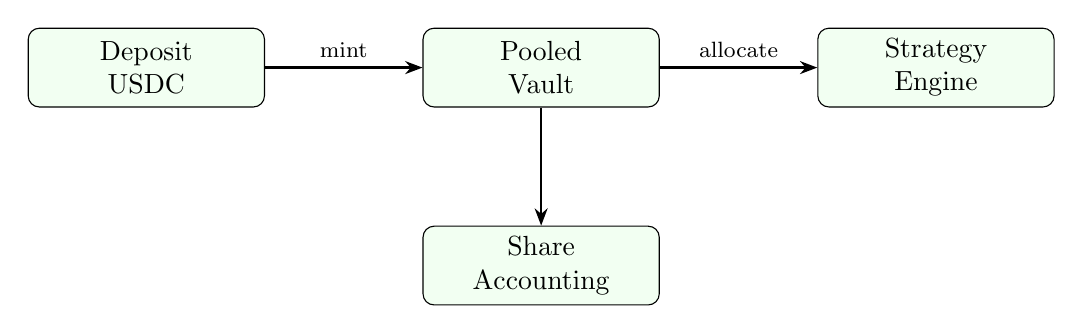
\begin{tikzpicture}[
  box/.style={rectangle, draw, rounded corners, minimum width=3cm, minimum height=1cm, align=center, fill=green!5},
  arrow/.style={-{Stealth[length=2.2mm]}, thick},
]

\node[box] (deposit) {Deposit\\USDC};
\node[box, right=2cm of deposit] (vault) {Pooled\\Vault};
\node[box, right=2cm of vault] (strategy) {Strategy\\Engine};
\node[box, below=1.5cm of vault] (shares) {Share\\Accounting};

\draw[arrow] (deposit) -- node[above] {\footnotesize mint} (vault);
\draw[arrow] (vault) -- node[above] {\footnotesize allocate} (strategy);
\draw[arrow] (vault) -- (shares);

\end{tikzpicture}
\caption{Vault deposit flow}
\end{figure}

\section{Share Accounting}

The vault uses share-based NAV accounting:

\begin{lstlisting}[language=Rust, caption={Core vault data structures}]
#[derive(Debug, Clone, Default)]
pub struct VaultShareState {
    pub total_shares: f64,
    pub user_shares: HashMap<String, f64>,
}

#[derive(Debug, Clone, Serialize, Deserialize)]
pub struct VaultStateResponse {
    pub cash_usdc: f64,
    pub nav_usdc: f64,
    pub total_shares: f64,
    pub nav_per_share: f64,
}

#[derive(Clone)]
pub struct PooledVault {
    pub db: Arc<VaultDb>,
    pub ledger: Arc<Mutex<VaultPaperLedger>>,
    pub shares: Arc<Mutex<VaultShareState>>,
}
\end{lstlisting}

\subsection{Deposit Flow}

\begin{lstlisting}[language=Rust, caption={Deposit implementation}]
pub async fn deposit(
    &self,
    wallet_address: &str,
    amount_usdc: f64,
) -> Result<VaultDepositResponse> {
    let wallet = wallet_address.trim().to_lowercase();
    
    // Validate inputs
    if wallet.is_empty() {
        return Err(anyhow!("wallet_address required"));
    }
    if !(amount_usdc.is_finite() && amount_usdc > 0.0) {
        return Err(anyhow!("invalid amount"));
    }

    let mut ledger = self.ledger.lock().await;
    let mut shares = self.shares.lock().await;

    // Calculate NAV and share price
    let nav_before = approximate_nav_usdc(&ledger);
    let nav_per_share = if shares.total_shares > 0.0 {
        (nav_before / shares.total_shares).max(1e-9)
    } else {
        1.0  // Initial share price
    };
    
    // Mint shares
    let shares_minted = amount_usdc / nav_per_share;
    
    // Update state
    ledger.cash_usdc += amount_usdc;
    shares.total_shares += shares_minted;
    *shares.user_shares
        .entry(wallet.clone())
        .or_insert(0.0) += shares_minted;

    // Persist to database
    self.db.upsert_state(
        ledger.cash_usdc, 
        shares.total_shares, 
        Utc::now().timestamp()
    ).await?;

    Ok(VaultDepositResponse { /* ... */ })
}
\end{lstlisting}

\subsection{Withdrawal Flow}

Withdrawals burn shares and return USDC:

\begin{equation}
\text{USDC}_{\text{withdrawn}} = \text{shares}_{\text{burned}} \times \frac{\text{NAV}_{\text{total}}}{\text{shares}_{\text{total}}}
\end{equation}

\textbf{Note:} Current implementation supports cash-only withdrawals. Position liquidation is not yet implemented---if cash is insufficient, the withdrawal fails.

\clearpage

\section{Paper Execution Adapter}

Before live deployment, all strategies execute through a paper adapter with realistic market simulation:

\begin{lstlisting}[language=Rust, caption={Paper execution configuration}]
#[derive(Debug, Clone)]
pub struct PaperExecutionConfig {
    /// Base latency in ms (+ random jitter)
    pub base_latency_ms: u64,         // Default: 150
    pub latency_jitter_ms: u64,       // Default: 200
    
    /// Slippage modeling
    pub slippage_bps_per_1k: f64,     // Default: 15 bps
    pub base_slippage_bps: f64,       // Default: 10 bps
    
    /// Fee structure
    pub fee_rate: f64,                // Default: 0.5%
    
    /// Fill simulation
    pub partial_fill_prob: f64,       // Default: 15%
    pub min_fill_ratio: f64,          // Default: 40%
    pub reject_prob: f64,             // Default: 2%
}
\end{lstlisting}

\begin{lstlisting}[language=Rust, caption={Paper execution trait}]
#[async_trait::async_trait]
pub trait ExecutionAdapter: Send + Sync {
    async fn place_order(&self, req: OrderRequest) -> Result<OrderAck>;
}

#[derive(Debug, Clone, Serialize, Deserialize)]
pub struct OrderRequest {
    pub client_order_id: String,
    pub token_id: String,
    pub side: OrderSide,
    pub price: f64,           // Limit price (0..1)
    pub notional_usdc: f64,   // Spend amount
    pub tif: TimeInForce,     // GTC, IOC, FOK
    pub market_slug: Option<String>,
    pub outcome: Option<String>,
}

#[derive(Debug, Clone, Serialize, Deserialize)]
pub struct OrderAck {
    pub order_id: String,
    pub filled_notional_usdc: f64,
    pub filled_price: f64,
    pub filled_at: i64,
    pub fees_usdc: f64,
    pub slippage_bps: f64,
    pub latency_ms: u64,
}
\end{lstlisting}

\clearpage

% =============================================================================
\chapter{Risk Management}
% =============================================================================

\section{Kelly Criterion Position Sizing}

The Kelly Criterion provides a mathematically optimal framework for position sizing:

\begin{equation}
f^* = \frac{bp - q}{b} = \frac{p(b+1) - 1}{b}
\end{equation}

Where:
\begin{itemize}
  \item $f^*$ = optimal fraction of bankroll to bet
  \item $b$ = decimal odds - 1 (net odds)
  \item $p$ = probability of winning (our estimate)
  \item $q$ = probability of losing ($1 - p$)
\end{itemize}

For Polymarket binary contracts with price $P$:
\begin{equation}
b = \frac{1}{P} - 1
\end{equation}

\subsection{Fractional Kelly}

Full Kelly is aggressive and can lead to high volatility. \BETTER{} uses \textbf{fractional Kelly} (default 0.25$\times$):

\begin{equation}
f_{\text{actual}} = f^* \times k_{\text{fraction}}
\end{equation}

\begin{lstlisting}[language=Rust, caption={Kelly criterion implementation}]
#[derive(Debug, Clone, Serialize, Deserialize)]
pub struct KellyParams {
    pub bankroll: f64,
    pub kelly_fraction: f64,    // 0.25 = quarter Kelly
    pub max_position_pct: f64,  // 0.10 = max 10% per trade
    pub min_position_usd: f64,  // $1 minimum
}

pub fn calculate_kelly_position(
    confidence: f64,
    market_price: f64,
    params: &KellyParams,
) -> KellyResult {
    // Calculate edge
    let edge = confidence - market_price;
    if edge <= 0.0 {
        return KellyResult::no_trade("No edge");
    }

    // Kelly formula
    let odds = (1.0 / market_price) - 1.0;
    let p = confidence;
    let q = 1.0 - p;
    let full_kelly = (p * odds - q) / odds;
    
    // Apply fractional Kelly and caps
    let actual_fraction = full_kelly
        .max(0.0)
        .min(1.0) 
        * params.kelly_fraction;
    
    let capped_fraction = actual_fraction
        .min(params.max_position_pct);
    
    let position_usd = params.bankroll * capped_fraction;
    
    if position_usd < params.min_position_usd {
        return KellyResult::no_trade("Below minimum");
    }
    
    KellyResult {
        position_size_usd: position_usd,
        full_kelly_fraction: full_kelly,
        actual_fraction: capped_fraction,
        edge,
        should_trade: true,
        skip_reason: None,
    }
}
\end{lstlisting}

\clearpage

\section{Guardrails and Limits}

Multiple layers of protection prevent excessive risk:

\begin{table}[H]
\centering
\begin{tabular}{@{}lll@{}}
\toprule
\textbf{Guardrail} & \textbf{Default} & \textbf{Purpose}\\
\midrule
Max position per trade & 10\% bankroll & Diversification\\
Max position per market & 2\% bankroll & Concentration risk\\
Max position per topic & 5\% bankroll & Correlation risk\\
Max total exposure & 15\% bankroll & Tail risk\\
Min notional & \$5 & Avoid dust trades\\
Max notional & \$250 & Liquidity protection\\
Cooldown per market & 30--300s & Prevent overtrading\\
Max LLM calls/day & 200 & Cost control\\
Max tokens/day & 300,000 & Cost control\\
\bottomrule
\end{tabular}
\caption{Risk guardrails}
\end{table}

\section{Vault Engine Configuration}

\begin{lstlisting}[language=Rust, caption={Vault engine configuration}]
#[derive(Debug, Clone)]
pub struct VaultEngineConfig {
    // Master switches
    pub enabled: bool,
    pub paper: bool,
    
    // FAST15M (deterministic Up/Down)
    pub updown_poll_ms: u64,           // 2000
    pub updown_min_edge: f64,          // 0.01
    pub updown_kelly_fraction: f64,    // 0.05
    pub updown_max_position_pct: f64,  // 0.01
    pub updown_shrink_to_half: f64,    // 0.35
    pub updown_cooldown_sec: i64,      // 30

    // LONG (LLM-bounded)
    pub long_enabled: bool,
    pub long_poll_ms: u64,             // 5000
    pub long_min_edge: f64,            // 0.02
    pub long_kelly_fraction: f64,      // 0.02
    pub long_max_position_pct: f64,    // 0.01
    pub long_min_trade_usd: f64,       // 5.0
    pub long_max_trade_usd: f64,       // 250.0
    pub long_cooldown_sec: i64,        // 300
    pub long_max_calls_per_day: u32,   // 200
    pub long_max_tokens_per_day: u64,  // 300000
    
    // LLM model ensemble
    pub long_models: Vec<String>,
}
\end{lstlisting}

\clearpage

% =============================================================================
\chapter{Frontend Terminal}
% =============================================================================

\section{Architecture}

The terminal provides a high-signal operator interface built with React 18 and TypeScript:

\begin{table}[H]
\centering
\begin{tabular}{@{}ll@{}}
\toprule
\textbf{Component} & \textbf{Purpose}\\
\midrule
\code{SignalFeed} & Real-time signal stream with filtering\\
\code{SignalCardCompact} & Dense HFT-style row display\\
\code{SignalInspectorDrawer} & Detail/performance/book/trade tabs\\
\code{SignalSearch} & Full-history + local fallback search\\
\code{TerminalHeader} & Navigation and status display\\
\bottomrule
\end{tabular}
\caption{Frontend component hierarchy}
\end{table}

\section{API Client}

Type-safe API communication with caching and timeout handling:

\begin{lstlisting}[language=TypeScript, caption={API client implementation}]
class ApiClient {
  private token: string | null = null;
  private cachedHeaders: Record<string, string> | null = null;

  private async fetch<T>(
    endpoint: string,
    options: RequestInit = {},
    timeoutMs: number = 15_000
  ): Promise<T> {
    const controller = new AbortController();
    let timedOut = false;
    
    const t = window.setTimeout(() => {
      timedOut = true;
      controller.abort();
    }, timeoutMs);

    try {
      const response = await fetch(`${API_URL}${endpoint}`, {
        ...options,
        signal: controller.signal,
        headers: {
          ...this.getHeaders(),
          ...(options.headers || {}),
        },
      });

      if (!response.ok) {
        const bodyText = await response.text().catch(() => '');
        const err: any = new Error(
          `API Error: ${response.status} ${response.statusText}`
        );
        err.status = response.status;
        err.body = bodyText;
        throw err;
      }

      return response.status === 204 
        ? null as T 
        : response.json();
    } catch (err: any) {
      if (err?.name === 'AbortError') {
        throw new Error(timedOut ? 'Request timed out' : 'Aborted');
      }
      throw err;
    } finally {
      window.clearTimeout(t);
    }
  }

  async getSignals(params?: {
    limit?: number;
    min_confidence?: number;
    before?: string;
    before_id?: string;
  }): Promise<{ signals: Signal[]; count: number }> {
    const query = new URLSearchParams();
    if (params?.limit) query.set('limit', String(params.limit));
    if (params?.min_confidence) 
      query.set('min_confidence', String(params.min_confidence));
    if (params?.before) query.set('before', params.before);
    if (params?.before_id) query.set('before_id', params.before_id);
    
    return this.fetch(`/api/signals?${query}`);
  }
}
\end{lstlisting}

\clearpage

\section{Search Implementation}

The terminal provides ``never dead'' search with automatic fallback:

\begin{enumerate}
  \item \textbf{Server mode (default)}: Full-history FTS5 search via \code{/api/signals/search}
  \item \textbf{Local mode (fallback)}: Substring match over loaded signal window
  \item \textbf{Auto-heal}: Periodically checks \code{/api/signals/search/status} and switches back to server mode when available
\end{enumerate}

\section{State Management}

Zustand provides lightweight, merge-aware state management:

\begin{lstlisting}[language=TypeScript, caption={Signal store with merge-by-id}]
const useSignalStore = create<SignalStore>((set) => ({
  signals: [],

  // Merge incoming signals by ID (REST + WS can overlap)
  setSignals: (incoming) => set((state) => {
    const byId = new Map(state.signals.map(s => [s.id, s]));
    
    for (const s of incoming) {
      const existing = byId.get(s.id);
      if (existing) {
        // Merge: prefer newer context_version
        byId.set(s.id, mergeSignal(existing, s));
      } else {
        byId.set(s.id, s);
      }
    }
    
    // Sort newest first, trim to 24h window
    const merged = [...byId.values()];
    merged.sort((a, b) => 
      new Date(b.detected_at).getTime() - 
      new Date(a.detected_at).getTime()
    );
    
    return { signals: trimToWindow(merged, 24 * 60 * 60 * 1000) };
  }),
}));
\end{lstlisting}

\clearpage

% =============================================================================
\chapter{Token Economics}
% =============================================================================

\section{Token Utility}

\tokenbetter{} serves as the access and alignment mechanism for the protocol:

\begin{itemize}
  \item \textbf{Terminal Access}: Holding above threshold enables terminal features
  \item \textbf{Vault Participation}: Staking enables deposits into automated strategies
  \item \textbf{Governance}: Future protocol parameter voting
  \item \textbf{Fee Sharing}: Performance fee distribution to stakers
\end{itemize}

\section{Token Distribution}

\begin{table}[H]
\centering
\begin{tabular}{@{}lrrp{5cm}@{}}
\toprule
\textbf{Allocation} & \textbf{\%} & \textbf{Tokens} & \textbf{Notes}\\
\midrule
Public Sale & 25\% & 250,000,000 & Unlocked at TGE\\
Liquidity & 15\% & 150,000,000 & Base/USDC LP, locked\\
Team & 20\% & 200,000,000 & 12mo cliff, 24mo vest\\
Treasury & 25\% & 250,000,000 & Ops, grants, partnerships\\
OpenServ Drop & 5\% & 50,000,000 & Unlocked\\
Programmatic & 10\% & 100,000,000 & Sold across FDV bands\\
\midrule
\textbf{Total} & \textbf{100\%} & \textbf{1,000,000,000} &\\
\bottomrule
\end{tabular}
\caption{Token allocation}
\end{table}

\section{Access Gate Schedule}

Access thresholds ratchet down as market cap increases:

\begin{table}[H]
\centering
\begin{tabular}{@{}lrrr@{}}
\toprule
\textbf{Phase} & \textbf{FDV Range} & \textbf{Required \tokenbetter{}} & \textbf{Est. Cost}\\
\midrule
1 & $<$\$10M & 100,000 & \$500--\$1,000\\
2 & \$10M--\$20M & 75,000 & $\sim$\$1,500\\
3 & \$20M--\$40M & 50,000 & $\sim$\$2,000\\
4 & $>$\$100M & 10,000 & $\sim$\$1,000\\
\bottomrule
\end{tabular}
\caption{Access gate ratchet schedule}
\end{table}

\section{Fee Model}

\begin{itemize}
  \item \textbf{Performance Fee}: 20\% of vault profits (assessed on withdrawal)
  \item \textbf{No Management Fee}: Only pay on profits
  \item \textbf{Execution Fee}: Nominal fee if using external routing (TBD)
\end{itemize}

\clearpage

% =============================================================================
\chapter{Roadmap}
% =============================================================================

\section{Phase 1: Foundation (Q1 2026)}

\begin{itemize}
  \item Token launch on Base
  \item Token-gated terminal access
  \item Paper vault with FAST15M strategy
  \item Signal detection pipeline (Dome + Binance)
  \item FTS5 full-history search
\end{itemize}

\section{Phase 2: Live Execution (Q2 2026)}

\begin{itemize}
  \item Live vault execution via Dome router
  \item Position tracking and reconciliation
  \item LONG (LLM) strategy activation
  \item Enhanced risk monitoring dashboard
  \item Mobile-responsive terminal
\end{itemize}

\section{Phase 3: Mirror Vault (Q3 2026)}

\begin{itemize}
  \item \tokenvbetter{} receipt token on Polygon
  \item Cross-chain deposit/withdrawal
  \item 24/7 receipt token liquidity
  \item Premium/discount arbitrage mechanism
  \item LP incentive program
\end{itemize}

\section{Phase 4: Expansion (Q4 2026)}

\begin{itemize}
  \item Additional prediction market venues
  \item Multi-strategy vault options
  \item Governance system activation
  \item Performance market exploration (HIP-3)
  \item API access for institutional users
\end{itemize}

\clearpage

% =============================================================================
\chapter{API Reference}
% =============================================================================

\section{Authentication}

All protected endpoints require JWT bearer token:

\begin{verbatim}
Authorization: Bearer <token>
\end{verbatim}

\section{Endpoints}

\begin{table}[H]
\centering
\footnotesize
\begin{tabular}{@{}lll@{}}
\toprule
\textbf{Method} & \textbf{Endpoint} & \textbf{Description}\\
\midrule
GET & /health & Health check (public)\\
POST & /api/auth/login & Username/password login\\
POST & /api/auth/privy & Privy wallet login\\
GET & /api/auth/me & Current user info\\
\midrule
GET & /api/signals & List recent signals\\
GET & /api/signals/search & Full-history FTS search\\
GET & /api/signals/search/status & Search index status\\
GET & /api/signals/enrich & On-demand signal enrichment\\
GET & /api/signals/stats & Signal statistics\\
\midrule
GET & /api/vault/state & Vault NAV and shares\\
POST & /api/vault/deposit & Deposit USDC, mint shares\\
POST & /api/vault/withdraw & Burn shares, withdraw USDC\\
\midrule
GET & /api/market/snapshot & Orderbook snapshot\\
GET & /api/wallet/analytics & Wallet performance data\\
POST & /api/wallet/analytics/prime & Warm analytics cache\\
\midrule
GET & /api/risk/stats & Risk manager statistics\\
GET & /ws & WebSocket upgrade\\
\bottomrule
\end{tabular}
\caption{API endpoint reference}
\end{table}

\section{WebSocket Protocol}

The WebSocket delivers real-time updates:

\begin{lstlisting}[language=TypeScript, caption={WebSocket message types}]
// Server -> Client
type WsServerEvent = 
  | { type: 'signal'; data: MarketSignal }
  | { type: 'signal_context'; data: SignalContextUpdate }
  | { type: 'pong'; timestamp: number };

// Client -> Server
type WsClientMessage =
  | { type: 'ping' }
  | { type: 'subscribe'; topics: string[] };
\end{lstlisting}

\clearpage

% =============================================================================
\chapter{Security Considerations}
% =============================================================================

\section{Authentication}

\begin{itemize}
  \item JWT tokens with configurable expiration
  \item Bcrypt password hashing (cost factor 12)
  \item Optional Privy wallet authentication
  \item Rate limiting on auth endpoints
\end{itemize}

\section{Secret Management}

\begin{itemize}
  \item All API keys loaded from environment variables
  \item No secrets in tracked source files
  \item Separate auth database from signal database
  \item Key rotation supported via env var reload
\end{itemize}

\section{Data Isolation}

\begin{itemize}
  \item Per-user share accounting
  \item Wallet address normalization (lowercase)
  \item Input validation on all endpoints
  \item SQL injection prevention via parameterized queries
\end{itemize}

\section{Operational Security}

\begin{itemize}
  \item Paper mode default for all strategies
  \item Feature flags for trading endpoints
  \item Graceful degradation on external API failures
  \item Health monitoring with auto-disable
\end{itemize}

\clearpage

% =============================================================================
\chapter{Risks and Disclaimers}
% =============================================================================

\section{Market Risks}

\begin{itemize}
  \item \textbf{Price Risk}: Prediction market positions can lose entire value
  \item \textbf{Settlement Risk}: Outcome disputes can delay or alter settlements
  \item \textbf{Liquidity Risk}: Thin orderbooks increase execution costs
  \item \textbf{Correlation Risk}: Multiple positions can move together
\end{itemize}

\section{Technical Risks}

\begin{itemize}
  \item \textbf{Software Bugs}: Despite testing, bugs may cause losses
  \item \textbf{API Failures}: External dependencies can become unavailable
  \item \textbf{Latency Degradation}: Network conditions affect execution
  \item \textbf{Model Error}: Signal confidence may be miscalibrated
\end{itemize}

\section{Regulatory Risks}

\begin{itemize}
  \item \textbf{Jurisdiction}: Prediction market legality varies by region
  \item \textbf{Token Classification}: Regulatory treatment may change
  \item \textbf{Compliance}: Future requirements may affect operations
\end{itemize}

\section{Not Financial Advice}

Nothing in this document constitutes investment, legal, or tax advice. \BETTER{} is experimental software. Users should:

\begin{itemize}
  \item Only risk capital they can afford to lose
  \item Conduct independent research
  \item Consult qualified professionals
  \item Understand all risks before participating
\end{itemize}

\clearpage

% =============================================================================
\chapter{Glossary}
% =============================================================================

\begin{description}[leftmargin=2.5cm, style=nextline]
  
  \item[Admissibility] The set of valid outputs from a bounded decision system. Invalid outputs trigger abstention rather than execution.
  
  \item[Alpha] Excess returns above a benchmark, typically from informational or execution advantages.
  
  \item[Alpha Decay] The reduction of exploitable edge as information is priced into markets, often measured in milliseconds for prediction markets.
  
  \item[Bounded Agent] An LLM-based decision system with deterministic constraints on output format and risk limits.
  
  \item[CLOB] Central Limit Order Book---a matching engine where bids and asks are prioritized by price-time.
  
  \item[Edge] The difference between estimated probability and market price: $\text{edge} = p_{\text{estimate}} - p_{\text{market}}$.
  
  \item[FTS5] SQLite's full-text search extension, used for efficient signal history queries.
  
  \item[Kelly Criterion] An optimal position sizing formula that maximizes expected logarithmic utility.
  
  \item[Mirror Vault] A cross-chain structure where deposits occur on one chain (Base) and liquid receipts trade on another (Polygon).
  
  \item[NAV] Net Asset Value---the total value of vault holdings divided by outstanding shares.
  
  \item[Paper Mode] Simulated execution that models latency, slippage, and fills without real capital at risk.
  
  \item[Prediction Market] A market where contracts settle on objective, verifiable outcomes.
  
  \item[Receipt Token] An ERC-20 representing proportional ownership of vault performance (e.g., \tokenvbetter{}).
  
  \item[Slippage] The difference between expected and actual execution price, caused by spread crossing and market impact.
  
  \item[WAL Mode] Write-Ahead Logging---a SQLite journal mode enabling concurrent reads during writes.
  
\end{description}

\clearpage

% =============================================================================
\chapter*{Conclusion}
\addcontentsline{toc}{chapter}{Conclusion}
% =============================================================================

\BETTER{} represents a new paradigm for prediction market participation. By combining:

\begin{itemize}
  \item \textbf{Institutional-grade infrastructure} with retail accessibility
  \item \textbf{Bounded AI decision systems} with deterministic safety
  \item \textbf{Paper-first validation} with path to live execution
  \item \textbf{Token-aligned incentives} with performance-based fees
\end{itemize}

The protocol aims to democratize access to the speed and sophistication that have historically been available only to professional trading operations.

The journey from paper to production is iterative and transparent. Every strategy, every trade, and every decision is auditable. The system is designed to fail safely, degrade gracefully, and improve continuously.

\vspace{1cm}

\begin{center}
\Large\textbf{Build the future of truth-settled markets.}\\[0.5cm]
\url{https://tradebetter.app}
\end{center}

\end{document}
